\documentclass{article}

\usepackage[english]{babel}
\usepackage[utf8]{inputenc}
\usepackage{amsmath,amssymb}
\usepackage{parskip}
\usepackage{graphicx}
\usepackage{listings}
\usepackage{float}
\lstset{
    numbers=left, 
    numberstyle= \tiny, 
    keywordstyle= \color{ blue!70},
    commentstyle= \color{red!50!green!50!blue!50}, 
    frame=shadowbox, % 阴影效果
    rulesepcolor= \color{ red!20!green!20!blue!20} ,
    escapeinside=``, % 英文分号中可写入中文
    xleftmargin=2em,xrightmargin=2em, aboveskip=1em,
    framexleftmargin=2em,
    breaklines=true,
    language=python,
    language=c++,
} 
% Margins
\usepackage[top=2.5cm, left=3cm, right=3cm, bottom=4.0cm]{geometry}
% Colour table cells
\usepackage[table]{xcolor}

% Get larger line spacing in table
\newcommand{\tablespace}{\\[1.25mm]}
\newcommand\Tstrut{\rule{0pt}{2.6ex}}         % = `top' strut
\newcommand\tstrut{\rule{0pt}{2.0ex}}         % = `top' strut
\newcommand\Bstrut{\rule[-0.9ex]{0pt}{0pt}}   % = `bottom' strut

%%%%%%%%%%%%%%%%%
%     Title     %
%%%%%%%%%%%%%%%%%
\title{CSCI803 Assignment}
\author{Yao Xiao \\ SID 2019180015}
\date{\today}

\begin{document}
\maketitle

%%%%%%%%%%%%%%%%%
%   Problem 1   %
%%%%%%%%%%%%%%%%%
\section{Problem 1}
\begin{lstlisting}
# Set N 
N = 8
ld = [0] * 30
rd = [0] * 30
cl = [0] * 30
  
def printSolution(board):  
    for i in range(N): 
        for j in range(N): 
            print(board[i][j], end = " ") 
        print()  
  
def solveNQUtil(board, col):  
      
    if (col >= N): 
        return True
          
    for i in range(N): 
          
        if ((ld[i - col + N - 1] != 1 and 
             rd[i + col] != 1) and cl[i] != 1): 
                   
            board[i][col] = 1
            ld[i - col + N - 1] = rd[i + col] = cl[i] = 1
              
            if (solveNQUtil(board, col + 1)): 
                return True
                  
            board[i][col] = 0 # BACKTRACK  
            ld[i - col + N - 1] = rd[i + col] = cl[i] = 0
              
    return False
      
def solveNQueue(): 
    board = [[0, 0, 0, 0, 0, 0 ,0, 0],  
             [0, 0, 0, 0, 0, 0 ,0, 0], 
             [0, 0, 0, 0, 0, 0 ,0, 0], 
             [0, 0, 0, 0, 0, 0 ,0, 0],
             [0, 0, 0, 0, 0, 0 ,0, 0],
             [0, 0, 0, 0, 0, 0 ,0, 0],
             [0, 0, 0, 0, 0, 0 ,0, 0],
             [0, 0, 0, 0, 0, 0 ,0, 0],
             ] 
    if (solveNQUtil(board, 0) == False): 
        print("Solution does not exist") 
        return False
    printSolution(board) 
    return True
      
solveNQueue()
\end{lstlisting}

\begin{figure}[H]
    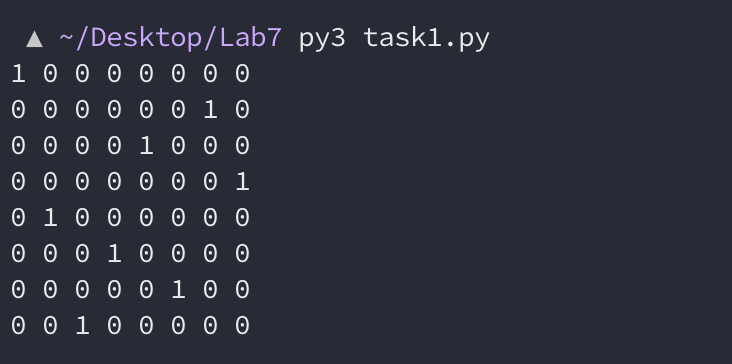
\includegraphics[width=1\textwidth]{Fig1}
\end{figure}

\section{Problem 2}
\begin{lstlisting}
#include <iostream>
#include "stdc++.h"

using namespace std;
#define N 4

struct Node {
    Node *parent;
    int pathCost;
    int cost;
    int machineID;
    int taskID;
    bool assigned[N];
};

struct comp {
    bool operator()(const Node *lhs,
                    const Node *rhs) const {
        return lhs->cost > rhs->cost;
    }
};

Node *newNode(int x, int y, bool assigned[],
              Node *parent) {
    Node *node = new Node;

    for (int j = 0; j < N; j++)
        node->assigned[j] = assigned[j];
    node->assigned[y] = true;

    node->parent = parent;
    node->machineID = x;
    node->taskID = y;

    return node;
}

int calculateCost(int costMatrix[N][N], int x,
                  int y, bool assigned[]) {
    int cost = 0;

    bool available[N] = {true};

    for (int i = x + 1; i < N; i++) {
        int min = INT_MAX, minIndex = -1;

        for (int j = 0; j < N; j++) {
            if (!assigned[j] && available[j] &&
                costMatrix[i][j] < min) {
                minIndex = j;

                min = costMatrix[i][j];
            }
        }

        cost += min;

        available[minIndex] = false;
    }

    return cost;
}

void printAssignments(Node *min) {
    if (min->parent == NULL)
        return;

    printAssignments(min->parent);
    cout << "Assign Machine " << char(min->machineID + '1')
         << " to Task " << min->taskID << endl;

}

// Finds minimum cost using Branch and Bound
int findMinCost(int costMatrix[N][N]) {
    priority_queue<Node *, std::vector<Node *>, comp> prq;

    bool assigned[N] = {false};
    Node *root = newNode(-1, -1, assigned, NULL);
    root->pathCost = root->cost = 0;
    root->machineID = -1;

    prq.push(root);

    while (!prq.empty()) {
        Node *min = prq.top();

        prq.pop();

        int i = min->machineID + 1;

        if (i == N) {
            printAssignments(min);
            return min->cost;
        }

        for (int j = 0; j < N; j++) {
            if (!min->assigned[j]) {
                Node *child = newNode(i, j, min->assigned, min);

                child->pathCost = min->pathCost + costMatrix[i][j];

                child->cost = child->pathCost +
                              calculateCost(costMatrix, i, j, child->assigned);

                prq.push(child);
            }
        }
    }
}

int main() {
    int costMatrix[N][N] =
            {
                    {13, 4,  7, 6},
                    {1,  11, 5, 4},
                    {6,  7,  2, 8},
                    {1,  3,  5, 9}
            };


    cout << findMinCost(costMatrix)
         << " is optimal min cost!";
    return 0;
}

\end{lstlisting}

\begin{figure}[H]
    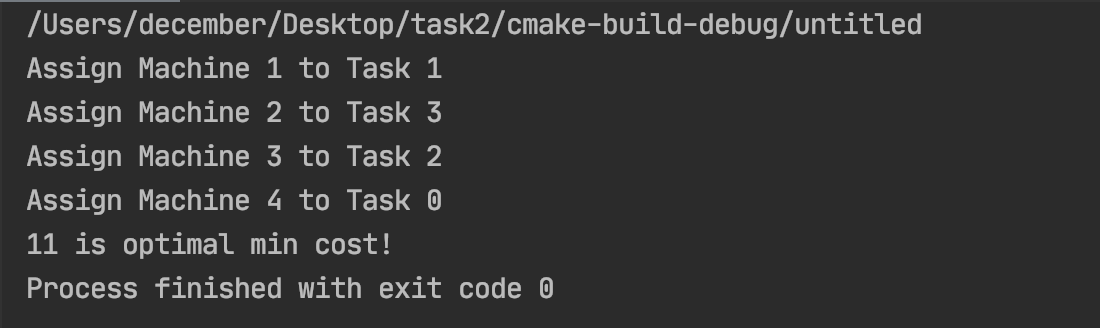
\includegraphics[width=1\textwidth]{Fig2}
\end{figure}
\end{document}
